\documentclass{webofc}
\usepackage[varg]{txfonts}   % Web of Conferences font

\usepackage[T2A]{fontenc} % указывает внутреннюю кодировку TeX
\usepackage[english]{babel}   %% загружает пакет многоязыковой вёрстки
\usepackage{color}
\usepackage{tasks}
\settasks {counter-format=(tsk[r])}
%\usepackage{exsheets}
\usepackage{array,graphicx,caption,paralist}
\newcommand{\er}{\textmd{EXPERTroot}}

\begin{document}
\title{Studies of the time properties of the NeuRad detector}

\author{\firstname{I.} \lastname{Muzalevsky}\inst{1,2,3}\fnsep\thanks{\email{ivanmuzalevskij@gmail.com}} \and
	\firstname{V.} \lastname{Chudoba}\inst{1,2}\fnsep\thanks{\email{chudoba@jinr.ru}} \and
	\firstname{A.} \lastname{Bezbakh}\inst{1} \and
	\firstname{I.} \lastname{Mukha}\inst{4} \and
	\firstname{O.} \lastname{Kiselev}\inst{4} \and
	\firstname{A.} \lastname{Fomichev}\inst{1} \and
	\firstname{S.} \lastname{Krupko}\inst{1} \and
	\firstname{D.} \lastname{Kostyleva}\inst{4} \and
	\firstname{A.} \lastname{Gorshkov}\inst{1} for the EXPERT project.
	% etc.
}
\institute{
	FLNR JINR Dubna, Russia; 
	\and
	Silesian University in Opava, Czech Republic;
	\and
	Dubna State University, Russia;
	\and
	GSI Helmholtzzentrum, Darmstadt
}
\abstract{%
	\color{red}
	This work is devoted to the calculation of the time resolution of the prototype of the neutron detector NeuRad. The NeuRad detector will be one of the EXPERT setup modules at Super-FRS. The experiments for calculation the time characteristics of the prototype of the NeuRad detector are described. The data processed methods were implemented into \er\, by which the simulation of the experiment was carried out.
}
%
\maketitle
%
\color{red}
\section{Intoduction}
Studying exotic nuclei is one of the most important fields in modern nuclear physics. Exotic nuclei are nuclei in which the ratio of the number of neutrons to the number of protons is much larger or smaller than in nuclei found in nature. In the case of exotic nuclei, such phenomena as neutron halo, soft mode of dipole excitation and others could be observed. As far as exotic nuclei are unstable there is a problem how to produce it. One of the most developed setup for production and separation   exotic nuclei in flight will be fragment separator Super-FRS at FAIR (Facility for Antiproton and Ion Research) \cite{diplom}. Project EXPERT (EXotic Particle Emission and Radioactivity by Tracking \cite{IMexpert}) dedicated to studying exotic nuclei properties is a part of program of the Super-FRS Experiment Collaboration. EXPERT setup consists of few modules each of which is intended to detect different decay products. 
\color{black}
%The EXPERT (EXotic Particle Emission and Radioactivity by Tracking) is a part of the physics program of the Super-FRS Experiment Collaboration. The experiments within EXPERT project are aimed at studies of the unknown exotic nuclear systems. 
%in the most-remote parts of the nuclear landscape which are characterized by the two borders between bound and un-bound nuclide (i.e. nuclear landscape beyond the proton and neutron drip-lines). 
%These experiments will use the first half of the Super-FRS as a radioactive beam separator and its second half as a high-resolution spectrometer. The exotic nuclei of interest will be produced in the middle focal plane of the Super-FRS. They are expected to decay in flight, and outgoing fragments (i.e., precursor-like decay products) will be tracked and then identified by the spectrometer part.


%\begin{enumerate}
%	\item Radiation-hard silicon strip detector (SSD). %These compact and universal beam detectors of the Super-FRS provide information on	time-of-flight, position and energy loss of ions, and it will be used for tracking of the secondary beam impinging the secondary target.
%	\item Microstrip silicon ($\mu$Si) tracking detectors. %These detectors are essential for applications of	tracking technique for studying of the radioactive decays-in-flight and providing information on trajectories of all charged decay products, which is sufficient for determination of half-life values in 	the range of 1 ps – 100 ns, as well as on decay energies and angular correlations of decay products.
%	\item The gamma-ray and light particles detector system GADAST (Gamma-ray Detectors Around Secondary Target). %It measures gamma-rays 	and light particles emitted instantaneously after secondary reaction. In the context of the proposal it	could allow to disentangle the decay channels with a heavy fragment resulting in an excited state (and 	thus instantaneously de-excited by gamma emission). The GADAST demonstrator has been successfully tested in the FRS experiment “Two-proton decay of 30 Ar”.
%	\item The OTPC (Optical Time Projection Chamber) for radioactivity studies by the implantation-decay method.
%	\item The NeuRad (Neutron Radioactivity) fine-resolution detector of neutrons. Together with $\mu$Si detectors, NeuRad will be able to provide precise information on angular correlations of decay neutrons with a charged fragment. This information will be used for calculations of the decay energy of the exotic nuclei \cite{IMexpert}.	
%\end{enumerate}

%paraenum clелать другой
%\begin{inparadesc}
%	\item[1] Radiation-hard silicon strip detector (SSD).
%	\item[2] Microstrip silicon ($\mu$Si) tracking detectors.
%	\item[3] The gamma-ray and light particles detector system GADAST (Gamma-ray Detectors Around Secondary Target).
%	\item[4]  The OTPC (Optical Time Projection Chamber) for radioactivity studies by the implantation-decay method.
%	\item[5]	The NeuRad (Neutron Radioactivity) fine-resolution detector of neutrons.
%\end{inparadesc}

These modules are:
\begin{inparaenum}[(i)]
	\item Radiation-hard silicon strip detector (SSD).
	\item Microstrip silicon ($\mu$Si) tracking detectors.
	\item The gamma-ray and light particles detector system GADAST (GAmma-ray Detectors Around Secondary Target).
	\item The OTPC (Optical Time Projection Chamber) for radioactivity studies by the implantation-decay method.
	\item The NeuRad (Neutron Radioactivity) fine-resolution detector of neutrons.
\end{inparaenum}

Additional important part of the EXPERT project is a framework for simulations of the experiments and processing of experimental data. For this purpose a framework EXPERTroot \cite{er} has been developed. %EXPERTroot is a framework for Monte-Carlo simulations of detector responses, event reconstruction and EXPERT experiment analysis.

This paper is dedicated to tests of a prototype of the NeuRad detector time properties and development of the EXPERTroot.

\section{Test of NeuRad timing properties}
Neutron detector NeuRad is aimed at providing precise information on angular correlations between nuclear-decay neutrons emitted from decay and heavy ion fragment which will be identified by Super-FRS beam diagnostic system. An information on angular correlations will be used to determine the decay energy of the precursor and its lifetime. Trajectories of a heavy ion and neutrons will be reconstructed by an array of $\mu$Si detectors and NeuRad detector respectively. %The trajectories of neutrons will be reconstructed from the data obtained by NeuRad.  %This number is determined by the low transfer momentum of the decay with energies expected in the range of 0.1-100 keV.  
NeuRad will be constructed from a large number of scintillating fibers ($\approx$10000 units). Each fiber will have a square cross section of 3$\times$3\,mm$^2$ and the length of 1\,m. Scintillating fibers will be grouped into bundles. 
The neutrons penetrating the detector will be mostly elastically scattered on protons (approximately 10\% of neutrons will be scattered on the carbon nuclei). In such a case recoil proton will produce a scintillation flash inside the fiber. The light emitted within the full reflection angle travels to the multi-anode photomultiplier tubes (MAPMT) located at the both ends of the fiber.
MAPMT's will be mounted to the bundles so that the area of each pixel corresponding to its anode will completely overlap the frontal surface of one fiber.

\begin{figure}[h]
	\center{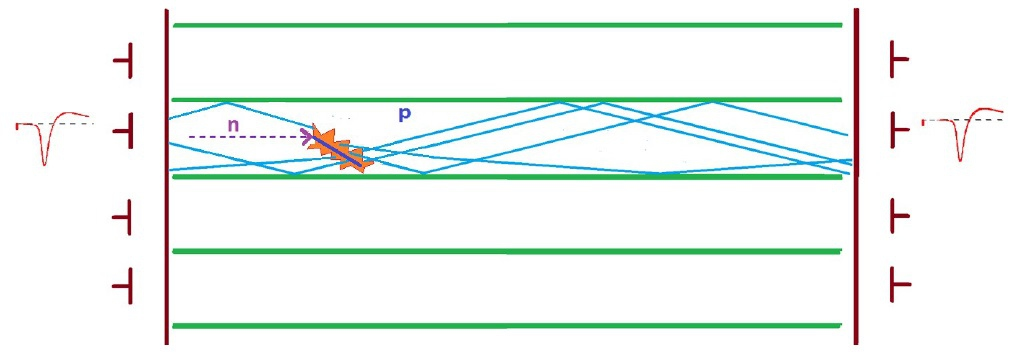
\includegraphics[width=1\linewidth]{neurad.png}}
	\caption{Illustration of the operational principle of the NeuRad detector. Each scintillating fiber will be coupled to one anode of the MAPMT. The neutron beam will penetrate through the frontal MAPMT's.}
	\label{ris:neuradPrinciple}
\end{figure}

In the course of planned experiments, NeuRad will be placed in 28 meters from secondary target so that the fibers will be oriented along the beam direction, see Fig.\ref{ris:neuradPrinciple}.
This is planned in order to provide sufficient efficiency of the detection and fine position resolution for neutrons with energies in lab system about $200-800$\,MeV.
With such a configuration the total angular acceptance of the detector will be about 12\,mrad.
Thus, the neutron beam will pass through the photomultiplier tubes before penetrating into the sensitive scintillating material.
Two coordinates, transverse to the direction of the beam, of the neutron interaction with the scintillating material will be obtained from the number of the fired fibers in which the scattering would be occurred.
The longitudinal coordinate will be determined from measurement of the time difference of the signals from two MAPT's located on the opposite sides of the detector.
The accuracy of determining the longitudinal coordinate of the interaction depends on the time resolution of the detector which is one of the significant characteristics of the intended NeuRad device.
%Time resolution is the accuracy of determining the time of interaction of a particle with the detector	.
For example, in order to obtain 20\,cm position resolution one has to ensure time-uncertainty better than 1\,ns.
Also it is important to define exactly the first neutron hit and following sequence of the signals induced in the detector material. This information allows to discriminate multi-neutron events from the multiple hits of a single re-scattered neutron.

%\section{Measurements}

The first investigation aimed to obtain timing characteristics of NeuRad detector was conducted recently in Flerov Laboratory of Nuclear Reactions JINR, Dubna. The NeuRad prototype was used for these test measurements. The sensitive part of the prototype was a bundle of 256 optical fibers made of scintillator plastic BCF-12. Each fiber was  3$\times$3\,mm$^2$ in cross section and 25\,cm long.
Two MAPMT's Hamamatsu H9500 were mounted to both sides of the bundle.


\begin{figure}[h]
	\centering
	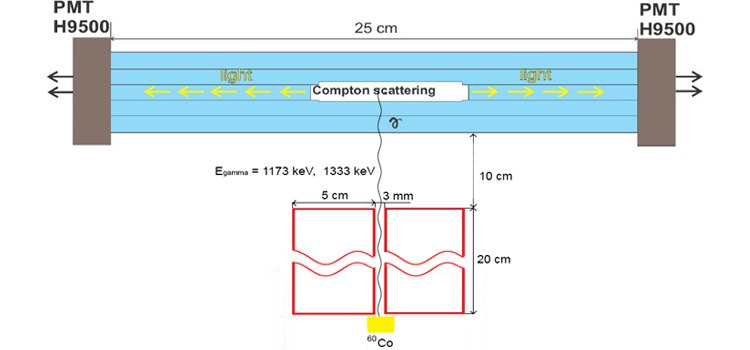
\includegraphics[width=1\linewidth]{NeuRadexperiment.png}
	\captionof{figure}{NeuRad measurements scheme. The prototype was irradiated by standart gamma source $^{60}$Co. The beam was focused at the geometrical center of the bundle and signals were collected by couple of H9500 MAPMT's.}
	\label{ris:neuradexp}
\end{figure}

This prototype was irradiated by collimated gamma beam with energies $E^{(1)}_{\gamma}$=1173\,keV and $E^{(2)}_{\gamma}$=1333\,keV emitted by $^{60}$Co as showed in Fig.~\ref{ris:neuradexp}. The beam was focused at the middle of the prototype. Signals obtained from MAPMT's was collected by the Tektronix oscilloscope MSO7354 and DRS4 evaluation board and its form was saved in binary file for each event.

\section{Simulations and data processing in EXPERTroot}
All conducted measurements were simulated in \er. For all simulations in \er\, method of simulating detector response \cite{er} is used.

The first step in simulation of the experiment was creating a virtual model of the setup described above.
The \er\, options allow to create any shape of detector model and fill in with any material. Created model of the experimental setup is showed in Fig.\ref{ris:sim}. 

\begin{figure}
	\centering
	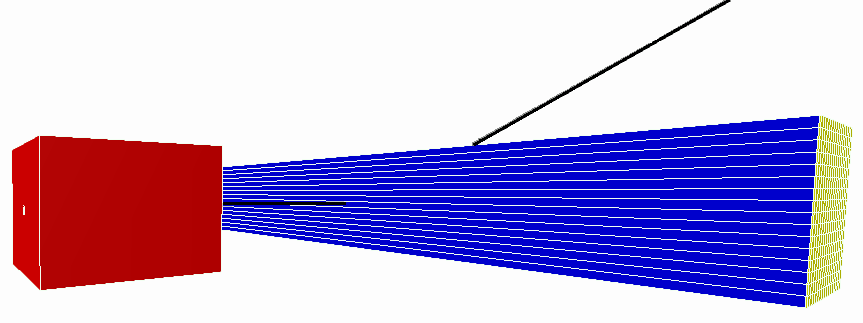
\includegraphics[width=\linewidth]{sim.png}
	\captionof{figure}{Simulations in  \er. Detector, collimator and PMT is depicted in blue, red and yellow colors respectively. The trajectory of the gamma particle is colored in black.}
	\label{ris:sim}
\end{figure}

The second step is transportation of the particles through the volume of the detector and obtaining of energy deposits of the particles at each step. This procedure is performing by well-known software GEANT4. And the last step of the simulation is the converting of energy deposits into detector signals.
In order to obtain plausible data all the physical effects occurring during the experiment were taken into account in simulations.
That's why such parameters as de-excitation scintillator time, quantum efficiency of the photocathode, the amplitude of the single electron signal, and others were calculated by analyzing of the experimental data or taken from used devices documentation.
%For simulations the conducted measurements method of simulation of the detector response \cite{diplom} was used. 

This method allowed to get the shape of the signals at the MAPMT anodes from all energy deposits of all NeuRad prototype fibers in the selected event. The MAPMT anode signal was calculated as a sum of the single photoelectron signals. 

A lot of data processing methods were developed and implemented into \er, for example well-known methods of obtaining signal time Constant Fraction Discriminator (CFD) and Leading Edge Discriminator (LED) \cite{diplom}.
The main advantage of using \er\, for data processing is a possibility to add any new processing algorithms the framework at any time. 
Implemented algorithms allowed to get such time and amplitude properties of the signal as rising time, Time-over-Threshold (ToT), anode charge and others. 

Methods of the \er\, allowed to get data from simulations of the same format as in experiment. That's why the same data processing algorithms were used for simulation and experimental data.

\color{red}
As the gamma beam was collimated the time resolution was calculated as a Full Width at Half Maximum (FWHM) of the distribution of the difference of the signal times from the opposite sides of the selected fiber. 
\color{black}
\section{Results}

The shapes of the signals obtained in the measurements and simulations were similar. 
The most successful method for calculation the time resolution was LED with selecting events by ToT.

At the Fig.\ref{ris:tausim} the distribution of the time difference of the signals from the opposite sides of one fiber is showed. Distribution obtained from experimental and simulated data colored in blue and red respectively.

\begin{figure}[h]
	\centering
	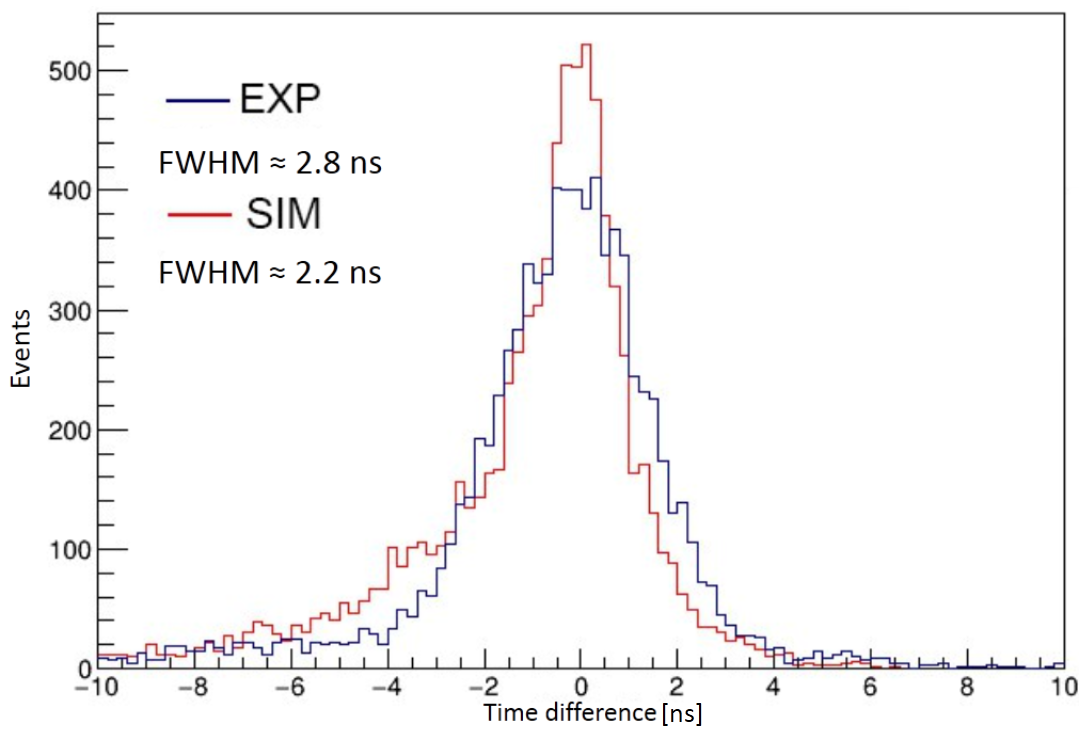
\includegraphics[width=0.8\linewidth]{tausim.png}
	\caption{The time difference distribution for experimental (blue) and simulation data (red). For obtaining time of the signal the leading edge algorithm was used.}\label{ris:tausim}
\end{figure}

Fig.\ref{ris:tausim} shows that for experimental data the obtained time resolution of the NeuRad prototype is 2.8\,ns. This time resolution corresponds to 56\,cm coordinate resolution. For simulation data the time resolution is 2.2\,ns which provides 44\,cm coordinate resolution.  

%Fig.\ref{ris:ampsim} shows the amplitude-time correlations for the simulated and experimental data at the left and right parts respectively.

%begin{figure}
%	\centering
%	\includegraphics[width=\linewidth]{ampsim.png}
%	\caption{Зависимость $\Delta\tau$ рассчитанное методом дискриминатора переднего фронта от заряда. Слева для моделированных, справа для экспериментальных данных }\label{ris:ampsim}
%\end{figure}

\section{Conclusion}

In the work the measurements of the time properties of the prototype of the neutron detector NeuRad were conducted.
Data processing algorithms for the detector were developed and implemented into the developing framework \er.

The time resolution of the prototype turned out to be 2.8\,ns which corresponds to 56\,cm of coordinate resolution.

All measurements were simulated using \er. It was found that the simulation results are in good agreement with the experimental. It confirms that options \er\, allows to simulate experiments with whole NeuRad detector.
Therefore, the results of this work are very important contribution to the development of the EXPERT project.

\section{Acknowledgement}	
RNF grant, LM and LTT grant, ICRF?

\begin{thebibliography}{999}
	
	\bibitem{diplom} SUPERFRS
	
	\bibitem{IMexpert} 
	Geissel, H., Kiselev, O., Mukha, I., et al., "Expert (exotic Particle Emission and Radioactivity by Tracking) Studies at the Super-Frs Spectrometer", 2015, Exotic Nuclei: EXON-2014 - Proceedings of International Symposium.
	
	\bibitem{er}
	http://er.jinr.ru/
	
	\bibitem{hm} 
	www.hamamatsu.com/
	
	\bibitem{crystals} 
	https://www.crystals.saint-gobain.com/
	
\end{thebibliography}

\end{document}